\begin{center}
    \section*{Практична частина}
\end{center}

Для дослідження методів, описаних у теоритичнії
частині, нами, на мові программування Python, було імплементовано усі вищезазначені алгоритми,
а саме:
\vspace{0.25cm}
\begin{enumerate}
    \item Метод Ньютона
    \item Квазіньютоновські методи:
    \begin{enumerate}
        \item SR1
        \item Broyden
        \item DFP
        \item BFGS
    \end{enumerate}
    \item Гука-Дживса
    \item Нелдера-Міда
    \item Генетичний алгоритм
\end{enumerate}

За допомогою цих алгоритмів ми будемо шукати
рішення безумовної задачі оптимізації \ref{eq:optimization_task}
для наступних функцій:

\begin{figure}[h!]
    % \hspace{-2cm}
    \begin{subfigure}{0.3 \textwidth}
        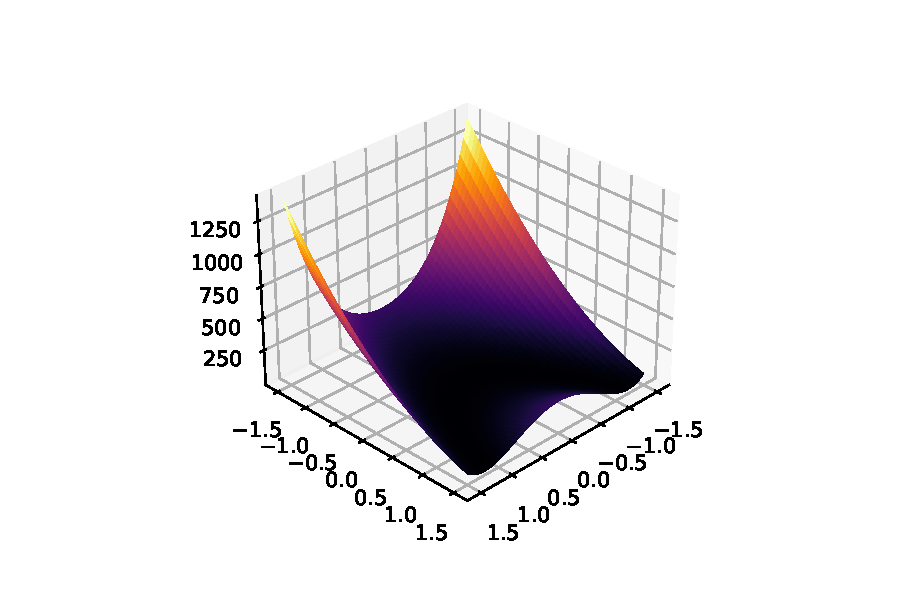
\includegraphics[width=1.5\textwidth,scale=3, trim=3.5cm 0 0 0]{assets/rosenbrock.pdf}
        \caption{Розенброка}
    \end{subfigure}
    \begin{subfigure}{0.3 \textwidth}
        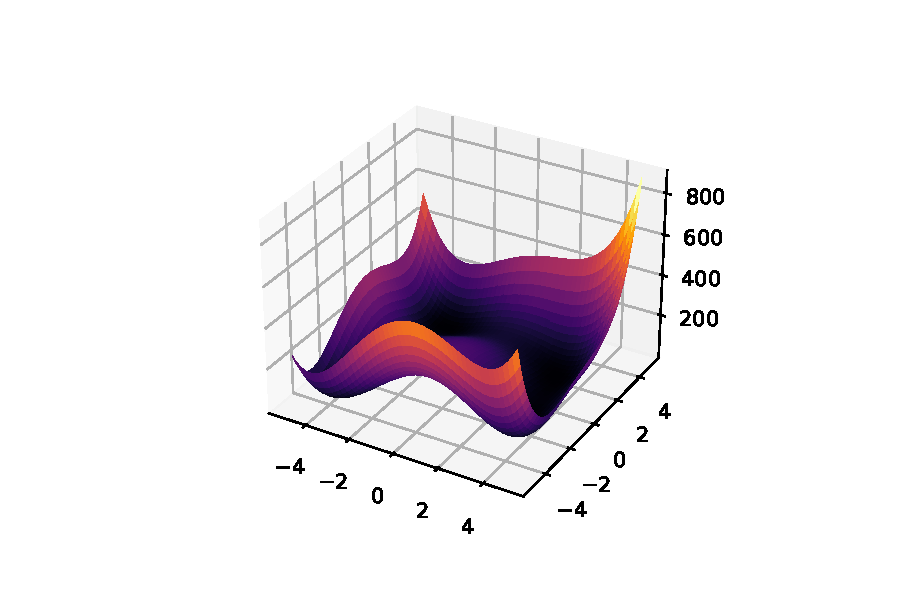
\includegraphics[width=1.45\textwidth, scale=3, trim=3.5cm 0 0 0]{assets/himmelblau.pdf}
        \caption{Хіммельблау}
    \end{subfigure}
    \begin{subfigure}{0.3 \textwidth}
        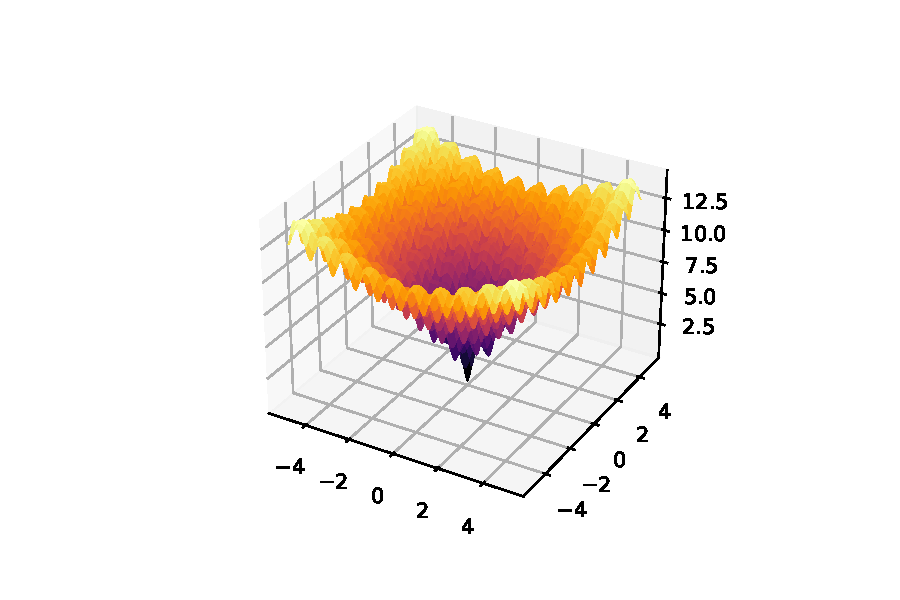
\includegraphics[width=1.5\textwidth, scale=3, trim=3.5cm 0 0 0]{assets/ackley.pdf}
        \caption{Еклі}
    \end{subfigure}
\end{figure}

\begin{enumerate}
    \item Функція Розенброка
    $$ f(x) = 100(x_2-x_1^2)^2 + (x_1-1)^2 $$
    \item Функція Хіммельблау
    $$ f(x) = (x_1^2 + x_2 - 11)^2 + (x_1 + x_2^2 - 7)^2 $$
    \item Функція Еклі
    $$ f(x) = -20 \exp{\left[-\frac{1}{5} \sqrt{\frac{x_1^2 + x_2^2}{2}}\right]} -
    \exp{\left[\frac{\cos(2 \pi x_1) + \cos(2 \pi x_2)}{2}\right]} + e + 20 $$
\end{enumerate}

\begin{table}[h!]
    \centering
    \begin{tabular}{|c|c|c|}
        \hline
        Функція & $x_{min}$ & $f(x_{min})$ \\
        \hline
        Розенброка & (1, 1) &
        \multirow{6}{*}{0} \\ \cline{1-2}

        \multirow{4}{*}{Хіммельблау} &
        (3, 2) & \\ \cline{2-2}
        & $\approx$ (-2.8, 3.13) &  \\ \cline{2-2}
        & $\approx$ (-3.78, -3.28) &  \\ \cline{2-2}
        & $\approx$ (3.58, -1.85) &  \\ \cline{1-2}

        Еклі & (0, 0) & \\
        \hline
    \end{tabular}
    \caption{Мінімуми досліджуваних функцій}
\end{table}


\pagebreak
\subsection*{Метод Ньютона}

\subsection*{Квазіньютоновські методи}

\subsection*{Метод Гука-Дживса}

\subsection*{Метод Нелдера-Міда}

\subsection*{Генетичний алгоритм}

\subsection*{Порівняння досліджуваних методів оптимізації}
\begin{table}[h!]
    \centering
    \begin{tabular}{|c|c|c|c|c|}
        \hline
        \textbf{Алгоритм} & $x_{01}$ & $x_{02}$ & \textbf{Критерій зупинки} & \textbf{Кількість ітерацій}  \\
        \hline

    \end{tabular}
    \caption{Порівняльна таблиця для функції }
\end{table}
